% Chapter Template

\chapter{Experiments} % Main chapter title

\label{Experiments} % Change X to a consecutive number; for referencing this chapter elsewhere, use \ref{ChapterX}

%----------------------------------------------------------------------------------------
%	SECTION 1
%----------------------------------------------------------------------------------------

\section{Experimental Setup}

This section provides a detailed description of the experimental environment, datasets, model architectures, evaluation metrics, and procedures used to evaluate Sarosh’s Perceptron Networks (SPNs) in comparison to traditional Multi-Layer Perceptrons (MLPs). These experiments aim to rigorously assess the performance of SPNs across multiple domains; images, tabular data, and language data, and varying complexity levels within each domain.
%-----------------------------------
%	SUBSECTION 1
%-----------------------------------
\subsubsection{Experimental Environment}
All our experiments were carried out with the following hardware specifications and software environment. Python was used for development. The hardware and software configurations are shown in Table \ref{tab:hardware} and \ref{tab:software} respectively.

\begin{table}[h!]
\centering
\caption{Hardware Specifications.}
\label{tab:hardware}
\begin{tabular}{| m{4cm} | m{6cm} |}
\hline
\textbf{Component} & \textbf{Details} \\
\hline
GPU & NVIDIA Tesla V100-PCIE GPU \\
GPU memory & 16GB \\
\hline
\end{tabular}
\end{table}

\begin{table}[h!]
\centering
\caption{Software Environment.}
\label{tab:software}
\begin{tabular}{| m{4cm} | m{4cm} |}
\hline
\textbf{Component} & \textbf{Version} \\
\hline
Python & 3.9.21 \\
PyTorch & 1.9.0 \\
CUDA & 11.8.0 \\
Transformers & 4.49.0 \\
Tensorflow & 2.10.0 \\
scikit-learn & 1.6.1 \\
Datasets & 3.3.2 \\
Matplotlib & 3.9.4 \\
\hline
\end{tabular}
\end{table}

\subsection{Datasets}

To address \ref{RQ5}, the experiments were structured across three distinct domains: images, tabular data, and language data. For each domain, two datasets were chosen. One, referred to as the simple variant, had fewer input features and training samples, while the complex variant had more. This approach allowed a comprehensive evaluation of SPN performance across varying complexity and data modalities.

For binary classification tasks, the number of classes was set to 2 as it allowed us to use the same optimizer (ADAM) and loss function (CrossEntropy Loss) as the multi-class classification tasks.

\subsubsection{Image Datasets}
For the image domain, the MNIST dataset served as the simpler variant. MNIST consists of 70,000 grayscale images of handwritten digits from 0–9, with 60,000 images allocated for training and 10,000 images reserved for testing. Each image is represented by 784 pixel features. 

The complex image dataset selected was CIFAR-10, which contains 60,000 RGB color images divided evenly into 10 classes—airplane, automobile, bird, cat, deer, dog, frog, horse, ship, and truck. CIFAR-10 is structured into 50,000 training images and 10,000 test images, each with 3,072 pixel features.

\subsubsection{Tabular Datasets}
In the tabular domain, the simple variant chosen was the Titanic dataset, which contains passenger information aimed at predicting survival during the Titanic disaster. Features include passenger class, gender, age, number of siblings or spouses aboard, number of parents or children aboard, fare amount, and embarkation port for a total of 7 input features. The dataset is composed of 712 training samples and 179 test samples, forming a binary classification task.

The complex variant selected was the Covertype dataset, which aims to predict forest cover types based on cartographic variables. The dataset includes 54 features, comprising 14 numerical and 40 binary indicators, representing various wilderness areas and soil types. This dataset contains approximately 88,000 training samples and 22,000 testing samples across 7 forest cover classes.

\subsubsection{Language Datasets}
For text-based tasks, the simple variant was the 20 Newsgroups dataset, comprising approximately 20,000 newsgroup documents categorized into 20 distinct topics such as politics, technology, and sports. The dataset is split into 13,000 training samples and 5,600 testing samples. 

The complex variant was the IMDB Reviews dataset, containing 50,000 movie reviews equally divided into 25,000 training and 25,000 test samples, each labeled with a positive or negative sentiment, making it a binary classification task. Text data in both datasets were standardized to 5,000 features using TF-IDF vectorization.

\subsubsection{Summary}

Across the tabular and language datasets, we selected a combination of simple and complex datasets: the Titanic dataset and the IMDB dataset for binary classification, and the Newsgroups dataset and the Covertype dataset for multi-class classification. This selection allows for a comprehensive evaluation of SPNs and MLPs across binary and multi-class classification tasks of varying complexity. Regression tasks were excluded from these tests to avoid introducing additional variables, ensuring a more focused and reliable comparison between MLPs and SPNs.

Table \ref{tab:dataSummary} outlines a summary of all the datasets used in our experiments.


\begin{table}[h!]
  \centering
   \begin{tabular}{|l|l|l|l|l|l|l|}
    \hline
    \textbf{Name} & \textbf{Domain} & \textbf{Variant} & \textbf{In size} & \textbf{Classes} & \textbf{Train Size} & \textbf{Test Size} \\
    \hline
    MNIST & Image & Simple & 784 & 10 & 60000 & 10000 \\
    CIFAR 10 & Image & Complex & 3072 & 10 & 50000 & 10000 \\
    Titanic & Tabular & Simple & 7 & 2 & 712 & 179 \\
    Covertype & Tabular & Complex & 54 & 7 & 88314 & 22079 \\
    Newsgroups 20 & Language & Simple & 5000 & 20 & 13192 & 5654 \\
    IMDB Reviews & Language & complex & 5000 & 2 & 25000 & 25000 \\
    \hline
  \end{tabular}
  \caption{Dataset Summary.}
  \label{tab:dataSummary}
\end{table}

%-----------------------------------
%	SUBSECTION 2
%-----------------------------------

\subsection{Model Architectures}
The following six model architectures were tested for each dataset. Since the experiments aim to observe the effects of varying levels of connectivity in Perceptron-based models, the total number of neurons were kept consistent throughout the models for each dataset. This ensured that the only variable across each model was their degree of inter-connectivity.

\begin{enumerate}
\item \textbf{Baseline MLP}: A conventional MLP was used as a control benchmark. Preliminary tests revealed that the best-performing MLP models achieved test accuracies exceeding 90\% across most datasets, but required extensive training times, leaving a minimal margin for improvements. Since the primary goal of the experiments was to assess the effects of varying neural connectivity, smaller MLPs that still performed adequately were selected, allowing the potential benefits of SPNs to be more clearly observed.
\item \textbf{Free Weights SPN}: An SPN that mirrors the layer structure of the baseline MLP, but with the addition of free weights; dense skip connections to all preceding layers. This model serves as a modified version of the baseline MLP, specifically designed to address \ref{RQ1}, enabling a direct examination of the effects of increased connection density.
\item \textbf{Mininal SPN}: To address \ref{RQ3}, the minimal SPN is a simplified two-layer architecture designed to maximize throughput while minimizing structural complexity. This model aims to optimize training time and allows us to investigate whether reducing the number of layers in a densely connected SPN can still deliver sufficient performance to justify the trade-off against multi-layer complexity.
\item \textbf{Minimal MLP}: are structurally similar to minimal SPNs, but they lack the denser connectivity inherent to SPNs. This model allows us to explore whether the potential benefits of minimal SPNs are exclusive to that architecture, or if similar advantages can be achieved with a similarly structured MLP. Like the baseline MLP and the Free Weights SPN, the minimal MLP and SPN models provide valuable insights into the distinctions between SPNs and MLPs, helping to address \ref{RQ1}.
\item \textbf{Maximal SPN}: are designed to maximize all connections between perceptrons for a given number of neurons. These models aim to address \ref{RQ2} by determining the upper performance threshold, while fully sacrificing efficiency and training time constraints in the pursuit of accuracy.
\item \textbf{Pruned Maximal SPN}: aim to preserve the performance of Maximal SPNs while optimizing training time. Maximal SPNs undergo a pruning process where zeroed-out weights are eliminated, leading to some neurons being disconnected. These disconnected neurons are subsequently merged into layers, enhancing the time complexity of the model. This approach addresses \ref{RQ6} and allows us to explore the possibility of optimizing maximal MLPs for time efficiency without compromising their higher performance accuracy.
\end{enumerate}

Figures \ref{fig:MLPWeights}, \ref{fig:fwSPNWeights} and \ref{fig:MaxSPNWeights} illustrate the differences between the baseline MLP, Free Weights SPN, and Maximal SPN model architectures while figures \ref{fig:minMLP} and \ref{fig:minSPN} highlight a direct comparison between minimal MLP and SPN architectures.

\begin{figure}[H]
    \centering
    \begin{minipage}{0.45\textwidth}
        \centering
        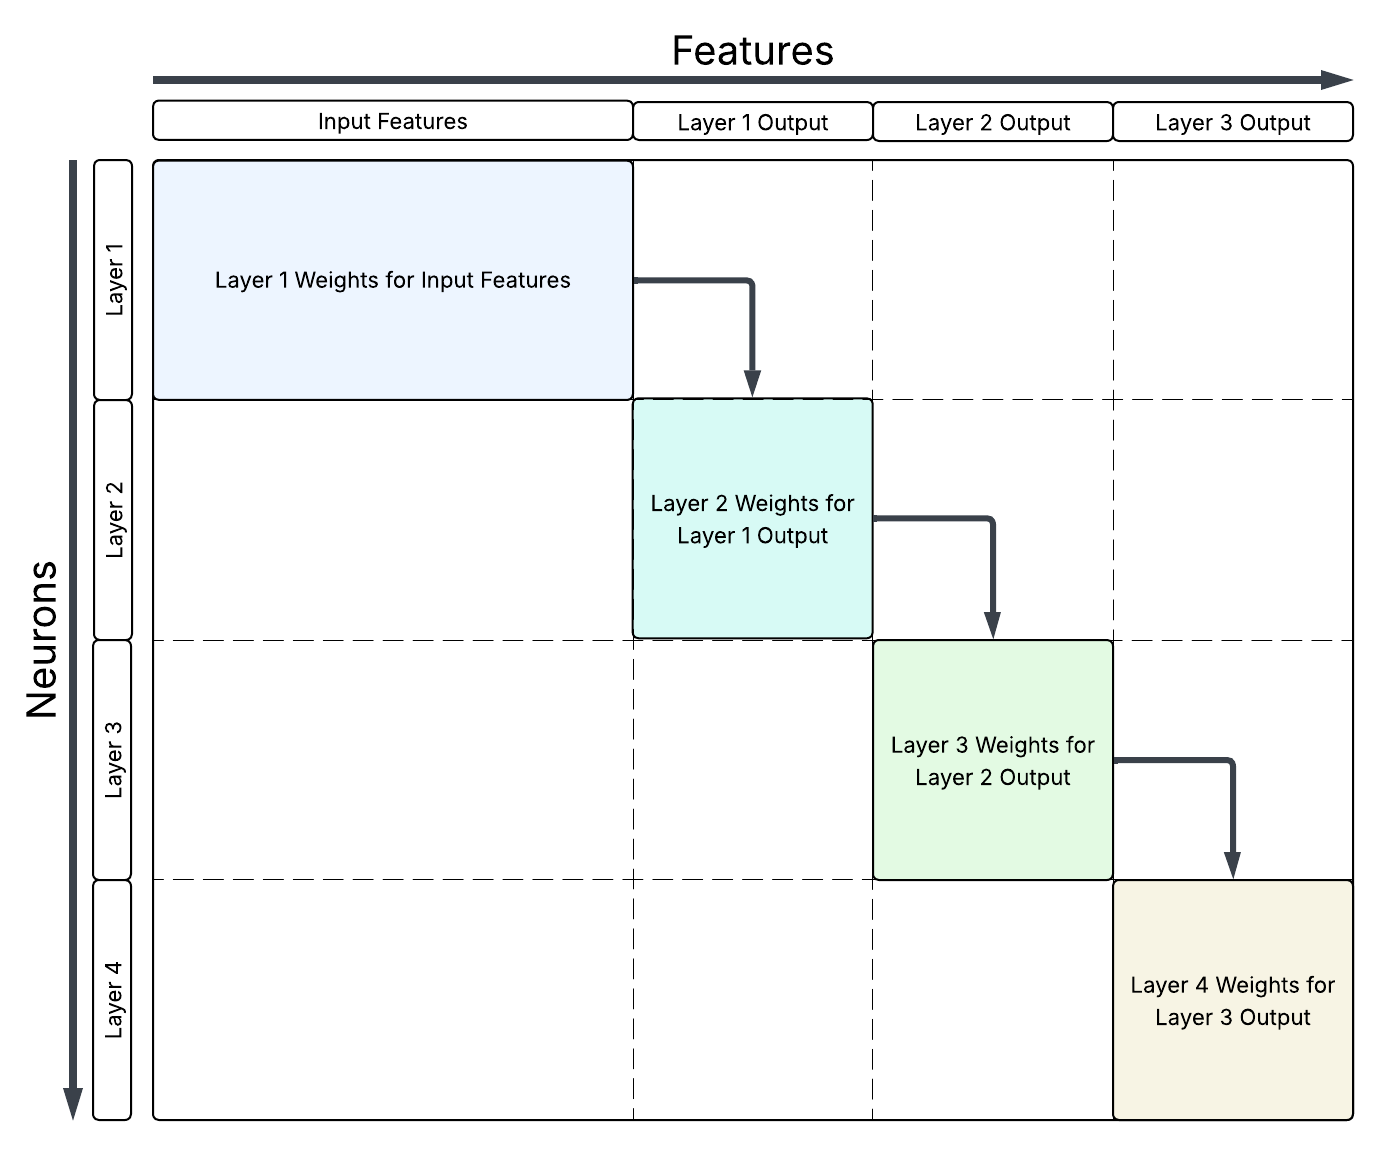
\includegraphics[height=0.25\textheight, width=\linewidth]{Figures/Experiments/MLP_weights.png} % first figure itself
        \captionsetup{width=\linewidth}
        \caption{MLP Weight Matrix}
        \label{fig:MLPWeights}
    \end{minipage}\hfill
    \begin{minipage}{0.45\textwidth}
        \centering
        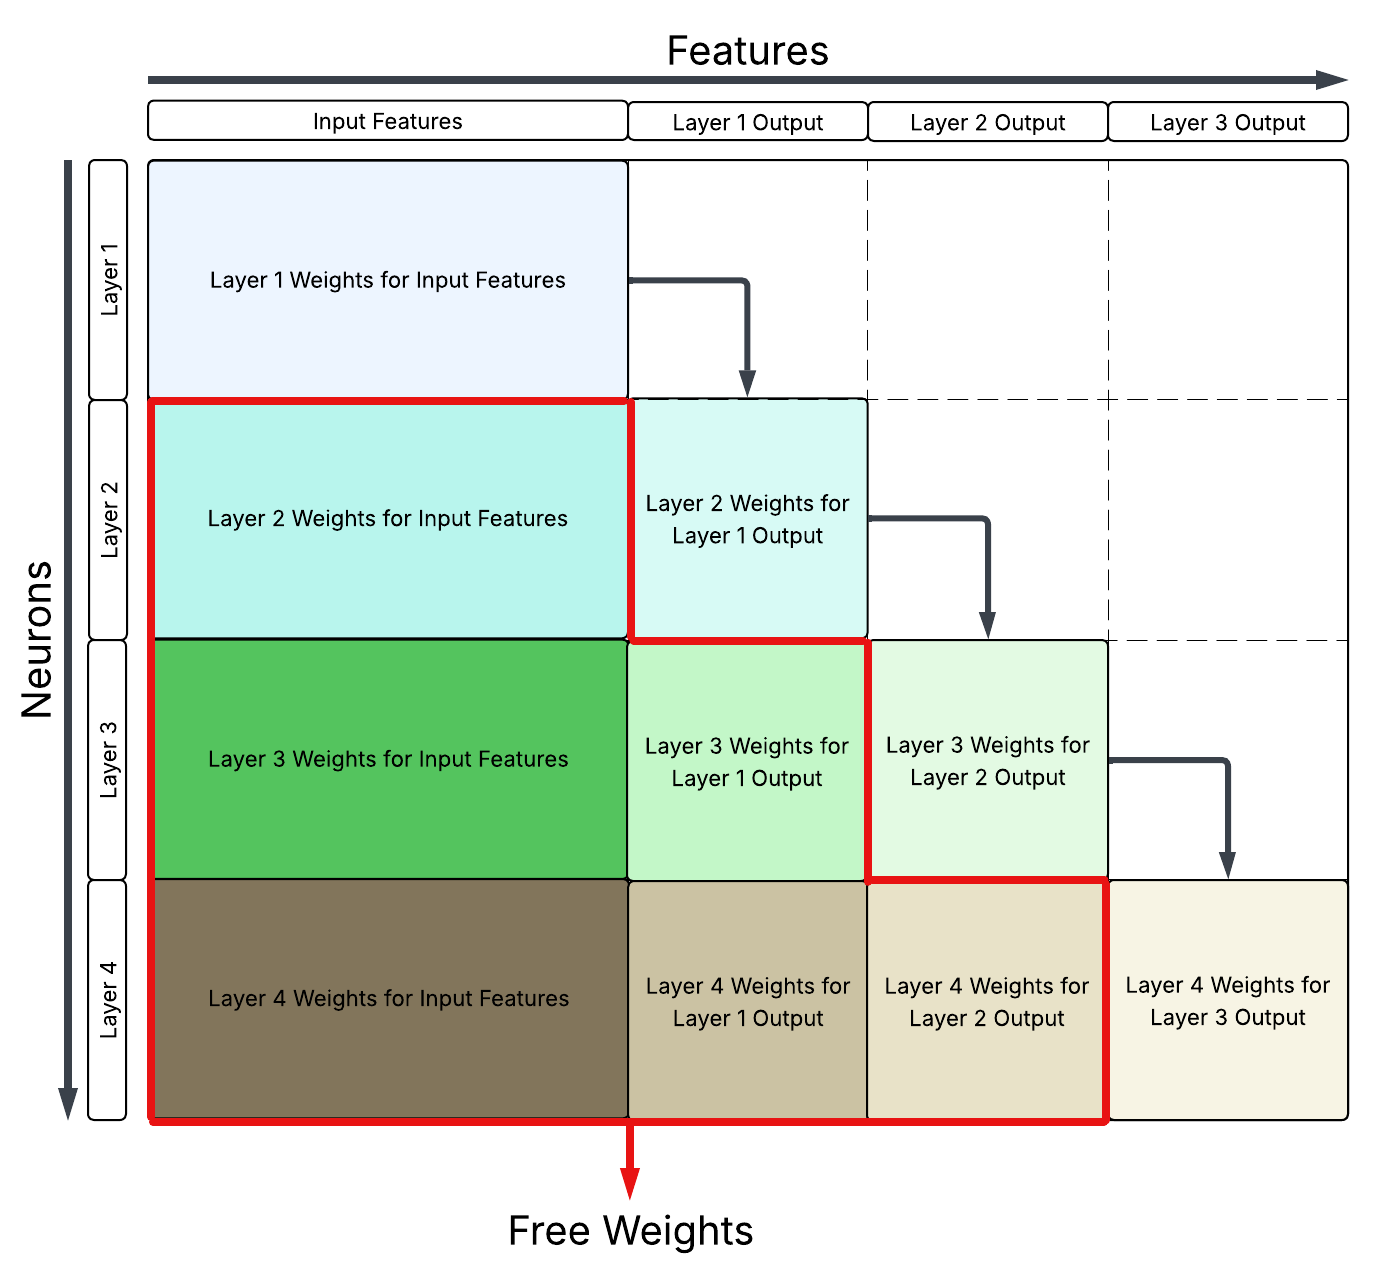
\includegraphics[height=0.25\textheight, width=\linewidth]{Figures/Experiments/Free_Weights_SPN_Weights.png} % second figure itself
        \captionsetup{width=\linewidth}
        \caption{Free Weights SPN Matrix}
        \label{fig:fwSPNWeights}
    \end{minipage}
    \begin{minipage}{0.7\textwidth}
        \centering
        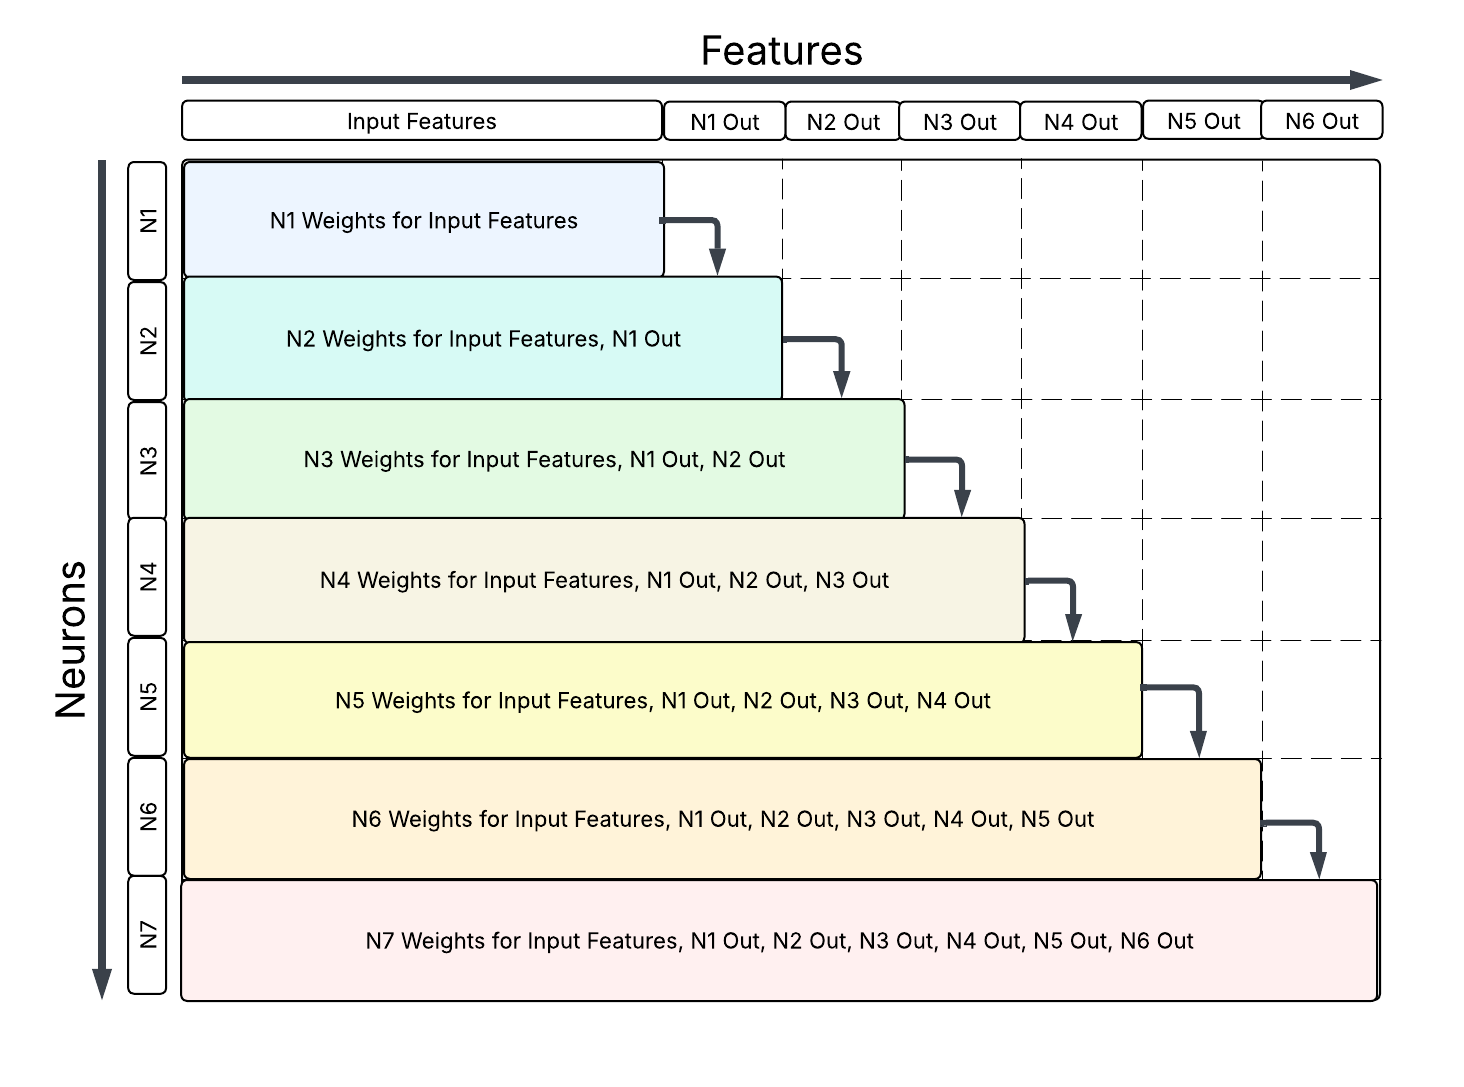
\includegraphics[height=0.3\textheight, width=\linewidth]{Figures/Experiments/Neuron_Based_Maximal_SPN_Weights.png} % first figure itself
        \captionsetup{width=\linewidth}
        \caption{Maximal SPN Weight Matrix}
        \label{fig:MaxSPNWeights}
    \end{minipage}\hfill
\end{figure}

\begin{figure}[H]
    \centering
    \begin{minipage}{0.45\textwidth}
        \centering
        \includegraphics[height=0.25\textheight, width=\linewidth]{Figures/Experiments/Minimal_MLP_weights.png} % first figure itself
        \captionsetup{width=\linewidth}
        \caption{Minimal MLP Weight Matrix}
        \label{fig:minMLP}
    \end{minipage}\hfill
    \begin{minipage}{0.45\textwidth}
        \centering
        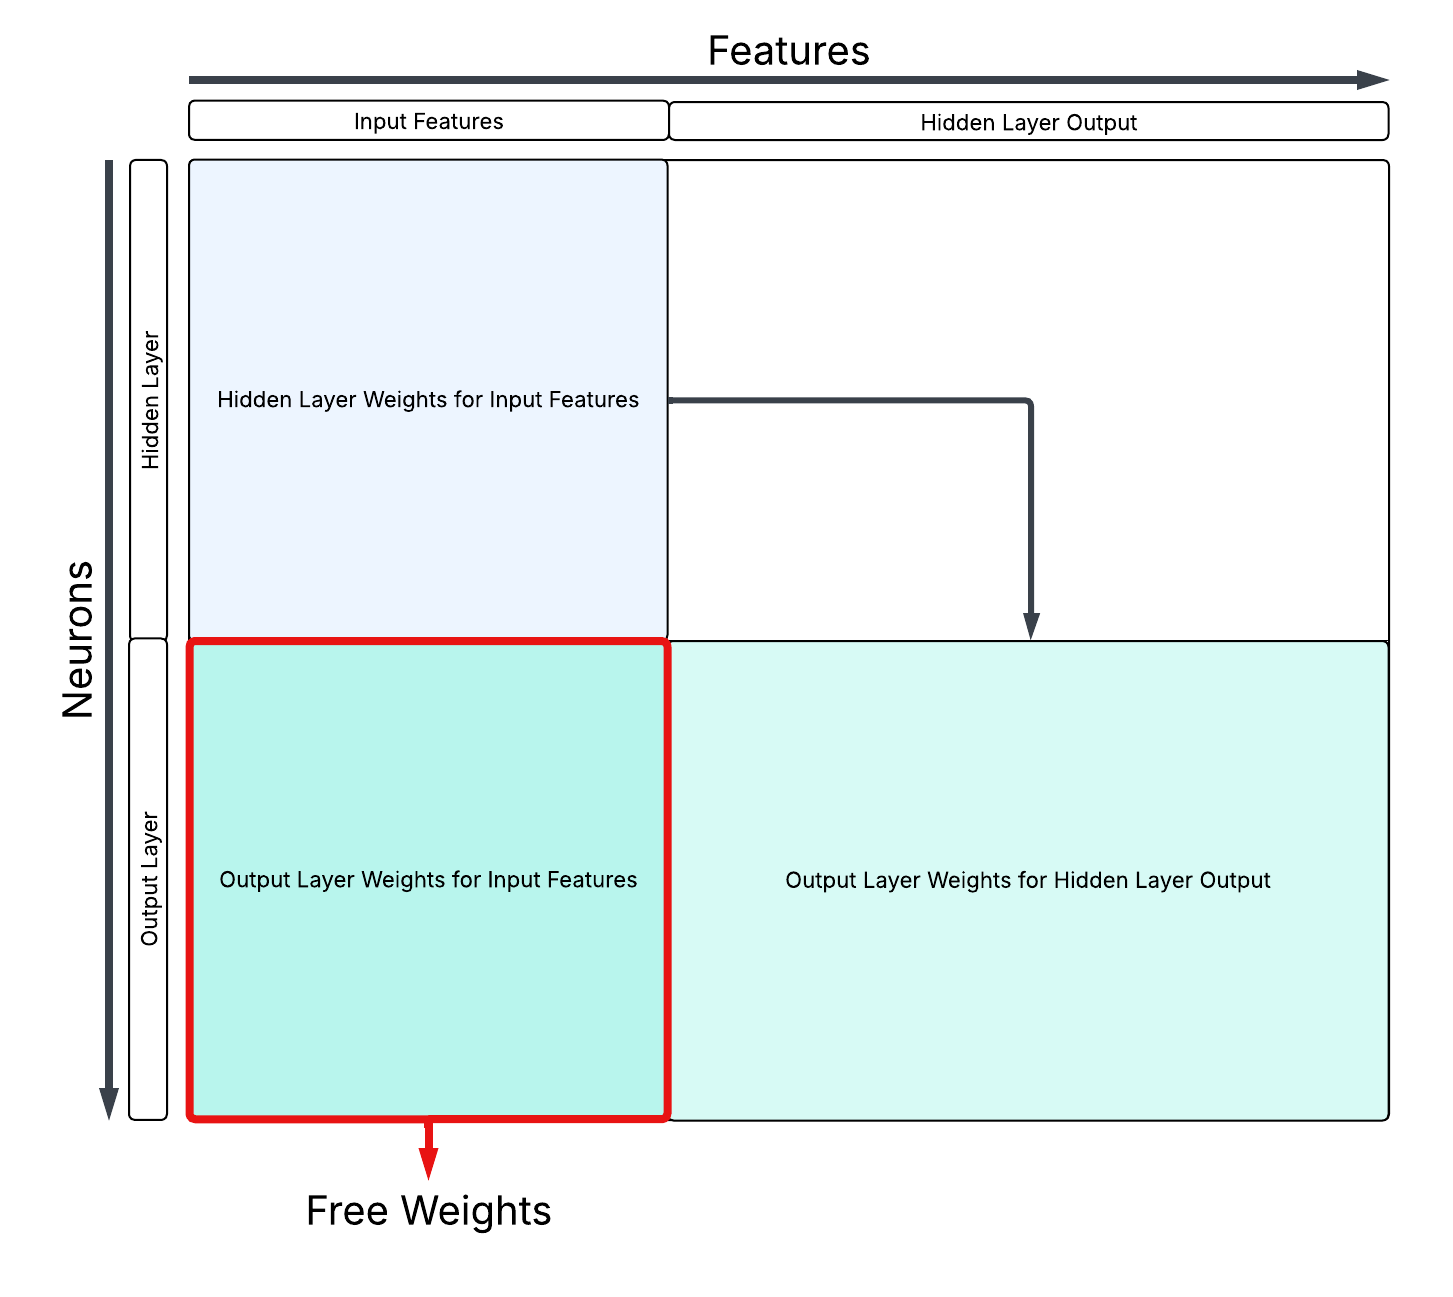
\includegraphics[height=0.25\textheight, width=\linewidth]{Figures/Experiments/Minimal_SPN_Weights.png} % second figure itself
        \captionsetup{width=\linewidth}
        \caption{Minimal SPN Weight Matrix}
        \label{fig:minSPN}
    \end{minipage}
\end{figure}


%----------------------------------------------------------------------------------------
%	SECTION 2
%----------------------------------------------------------------------------------------

\section{Experimental Procedure}

Each model was trained systematically over multiple epochs, with training time per epoch, training time per mini batch, average ttraining accuracy, training loss, test accuracy, and test loss recorded at each epoch.

Hyperparameters were fine-tuned through preliminary experimentation to identify optimal learning rates and batch sizes, with the goal of minimizing overfitting while maximizing training efficiency. The final set of hyperparameters enabled a robust comparative analysis across different architectures.

This experimental setup allowed for a comprehensive evaluation of the relative performance and potential advantages of SPNs over traditional MLPs, providing valuable insights across a range of domains and levels of complexity.

\subsection{Metrics}
Model performance on each dataset was evaluated using the following metrics:
\begin{enumerate}
\item \textbf{Parameter Count}: The total number of trainable parameters (weights and biases) in the model. It reflects the internal connectivity of the model.
\item \textbf{Best Test Accuracy}: The highest accuracy achieved on the testing dataset across all epochs.
\item \textbf{Time To Best Test Accuracy}: The cumulative training duration required to reach the epoch where the highest test accuracy was observed.
\item \textbf{Training Efficiency}: The ratio of the best test accuracy to the total training time required to achieve that accuracy. This metric demonstrates how quickly the model reaches its optimal performance and how effective that peak performance is.
\item \textbf{Area Under Curve (AUC) Efficiency}: The area under the test accuracy-time curve, reflecting how rapidly the model achieves high accuracy levels.
\item \textbf{Throughput Efficiency}: The ratio of the best test accuracy achieved to the average training time per epoch. This metric indicates the model's computational throughput and its effectiveness in achieving high performance with that throughput.
\end{enumerate}

In addition to evaluating model performance on each dataset, several other aspects were considered.

\begin{enumerate}
\item \textbf{Baseline MLP architecture}: The architecture for the baseline MLP was described.
\item \textbf{Total Neuron Count}: The total number of neurons (kept consistent across all models) was noted.
\item \textbf{Batch Size and Training Epochs}: Since both metrics can affect training time, they were kept consistent across all models.
\item \textbf{Pruning time for pruned maximal SPNs.}
\item \textbf{Number of layers before and after pruning.}
\item \textbf{Pruning effectiveness}: This was measured as the ratio between the mean epoch time of the max\_spn and the mean epoch time of the pruned\_spn. It reflects how fast the pruned\_spn is compared to the max\_spn.
\end{enumerate}

Together, these metrics enable us to address \ref{RQ4} and perform a comprehensive analysis of SPNs versus MLPs, considering time complexity, space complexity, and performance accuracy.